\documentclass[12pt]{article}
\usepackage[utf8]{inputenc}
\usepackage[margin = 1.03in]{geometry}
\usepackage{graphicx}
\title{Anatomy of a Disaster - Loma Prieta}
\author{Ian Gallmeister}
\date{April 2016}

\linespread{1.6} %for double spacing
%\linespread{1.3} %for 1.5 spacing

\begin{document}

\noindent Ian Gallmeister \\
Geography of Environmental Hazards \\
Anatomy of a Disaster \\
April 2016

\begin{center}
\large \textsc{\underline{loma prieta, california, and earthquake preparedness}} 
\end{center}

\vspace*{2em}

{\centering \section*{Abstract}}
Californians live on unstable ground.  The state straddles the boundary between the Pacific and North American plates, making life unpredictable for its residents.  People’s lives were turned upside down many times in the 20th century, and that will continue into the 21st.  One hotbed for this unpredictability is the Bay Area - one of the state’s population centers.  We will look at the qualities that make the Bay Area specifically vulnerable, the process of rebuilding, and preparation for the next big quake, focusing on Loma Prieta as a case study.

\vspace*{2em}

\section*{Introduction}
The time is about five in the evening, and game three of the World Series is about to start. People are finding their seats at Candlestick Park outside San Francisco.  Many others are at home or work or a bar to watch the game.  The Giants are down two games to none against the A's.  All of a sudden, everything starts shaking - hard.  Fifteen seconds later, everything is still again.  The earthquake is not uncommon in California, though the magnitude was.  This was the famous Loma Prieta earthquake on the 17th October 1989.  Though everybody remembers the big quakes, they are incredibly common.  From the 17th through the 23rd March 2016, California and Nevada experienced a collective 742 earthquakes (SCEDC).  To add some context, 742 quakes is about 45\% of global quakes for that week. (USGS).  Most of these earthquakes go unnoticed, but residents need to be prepared for what can and will eventually happen - another large quake disrupting their lives.  This earthquake was a huge disruption in the Bay Area and its surrounding environs.  How big was this disaster?  What caused it and other earthquakes to be so significant?  And how has California recovered from this one and prepared for the next?

\section*{Magnitude}
In California and the Bay Area in particular, faults are a significant source of issues.  In addition to the obvious earthquakes and aftershocks, there is a network of minor faults damping tremors.  Although this damping is incredibly beneficial, it decreases earthquake predictability and can lead to ground creep issues throughout the region.

Although the San Andreas Fault can have some very large earthquakes, physics limits the magnitude by the length and depth of the fault.  It is deep and long, and it hasn't breached along the full length of the fault, though its maximum magnitude seems to be about 8.1 (Lin \textrm{II}).  In comparison, one of the largest earthquakes on record is a magnitude 9.5 quake in Chile where the whole shallow fault (longer than the San Andreas) breached. Additionally, a magnitude 12 quake would require a fault longer than the circumference of the earth (Earthquake Facts).

Although there is a magnitude limit, the damage to fix in the aftermath of an earthquake is much less limited.  This will depend on population density, building age, and a host of other factors.  Additionally, the epicenter of an earthquake will have a significant effect.  In the case of the Loma Prieta quake, the epicenter was located in the Forest of Niscene Marks, a state park a little south of the Bay Area proper, near the sleepy town of Aptos.  Despite its relative remoteness, Loma Prieta managed to collapse many highways in San Francisco, including one part of the Bay Bridge connecting the City with Oakland.  Unlike the American East Coast, California's ground is highly fractured around faults, so tremors are more effectively dampened by distance than elsewhere.  Therefore, moving the point of maximum force closer to populations can render people significantly more vulnerable.  

This faultline spidering is a double edged sword.  While it is very useful for tremor damping, it can also make it difficult predict which fault will rupture and where aftershocks may happen.  In the case of Loma Prieta, there was a rather significant magnitude 4.7 aftershock in the Blossom Hill Fault two hours after the main quake. (How Close)  Blossom Hill is a short four and a half kilometer fault with just one known earthquake to its name located about fifteen miles from the epicenter of Loma Prieta.  The chance that it would be the source of such a significant aftershock given the number of longer, more significant faults in the area was rather small, yet it let loose with surprising strength.

In addition to decreasing quake predictability, the network of faults also experience creep.  Throughout the region, streets and sidewalks are cracked where the ground has shifted over the past decades.  One of the most prominent examples is Hollister's DeRose Winery whose main building was built on top of a fault.  Since 1988, one side of the building has shifted about eighteen inches from the other side.  Doorways are unusable, and there are cracks extending through the floor. Eventually, this cost the owners \$50,000 to retrofit the building to shift with the fault to prevent further damage to the property.  (Audi)

\section*{Causes}
So why are there so many earthquakes in California?  And why did so many people decide to live there?  Most importantly, what makes the aftereffects so large?  It is clear that nobody will stop California from shaking, so we must ask why people decided to put themselves in the vulnerable position of moving there.  There are a wide array of factors leading to this from fertile farmland to film studios to the tech industry.  However, the most important one is probably the gold rush.

When gold was discovered at Sutter's Mill in 1848, the news set off a population boom in the state.  This gold was unlike many previous ones in that the gold had made its way to the surface and was found with minimal effort.  As men flooded into the state to seek their fortunes, they were given a moniker - the 49ers.  Their port of entry?  San Francisco.  In fact, as more and more ships arrived in the bay and were abandoned by a riches-seeking crew.  Enterprising people saw an opportunity and filled in much of the bay to create land around these abandoned ships to use as shops.  By the time Loma Prieta happened, those ships had long been destroyed and replaced with more conventional buildings, and the area had been renamed as the Marina District.  This area, along with other filled-in areas like a lake right at the middle of the Mission District experienced the worst damage during the Loma Prieta quake, and could still experience significant difficulties in subsequent earthquakes. (Smith)

After the gold rush, many people stayed in California, and one of the main ways by which people employed themselves was agriculture.  California has a long growing season, and the soil of the central valley is very fertile, which has led to the state becoming the largest agricultural producer in the United States. (California Central Valley).  Those farms needed workers to manage the fields and levee system keeping many farms from being flooded, so there was opportunity for people throughout the valley to stay and farm after the gold had largely played out.  Here, the main danger from earthquakes comes in the form of levees which were built as giant dirt walls surrounding boulders to keep water out.  While gophers can cause breaches on their own, large quakes make farmers nervous that their island wall may suffer a destabilized levee and be breached.  The consequences of this event tend to be large, expensive, and impressive.  Some farms are abandoned in the face of these odds, and others stll have the rusty remains of farm equipment caught up in the breach sitting around their fields.

More recently, there has been a huge influx of workers to the Silicon Valley, formerly an agricultural area called the Valley of The Heart's Delight.  After the president of Stanford University put up some venture capital money to support Lee de Forest's invention of the vacuum tube.  A few decades later, Stanford Professor Frederick Terman encouraged his students to work and start companies locally.  This led to the foundation of Hewlett-Packard, and soon other companies started their own offices in the vicinity of Palo Alto. (Silicon Valley History)  The presence of so much industry in a small area has led to a multi-decade construction boom throughout Santa Clara and the surrounding environs.  An unforseen side effect of many towns existing on top of faults is the construction of homes and businesses right on top of faults.  There isn't unlimited bedrock upon which to build on as well.

Farther south, the LA area is known for the movie business, and much of LA is built around there.  As telecommuting becomes more and more common, many would-be Silicon Valley workers have relocated to the Los Angeles area in search of a culture more befitting their personalities.  Although movies are a huge draw, that isn't nearly enough to make LA the second largest metropolitan area in the United States.  Those honors go to consumer electronics imports and the aerospace industry.  LAX, the Los Angeles International Airport, is the main port of entry for small, luxury goods entering North America from China.  iPods assembled by Hon Hai Precision, Laptops from Lenovo, and many other items arrive in the US via LAX making these cargo shipments extremely valuable. (Kasarda \& Lindsay)  And during the Cold War, 25\% of all American aerospace jobs were based in California with 60\% of California's aerospace workers based in LA County with companies like Douglass Aircraft (now part of Boeing) based in Long Beach.  Although Southern California experienced a recession after the fall of the Soviet Union and no longer holds such a prominent position among the aerospace industry, it is still a key player in the local economy. (The Aerospace Industry)

Despite hiccups and shifts in dominant industries, it is clear that there are many reasons to move to California without even mentioning the gorgeous beaches, forests, and temperate weather.

\section*{Vulnerability}
Although many people live in California, and the building code compensates for earthquake risk, there are still many areas in which the state is vulnerable.  The most concerning is water.  In a report released in March 2016, the city of Los Angeles identified its main vulnerabilities, one of which was water calling it the most vulnerable utility due to age and a vulnerability to many types of damage. (Los Angeles Mayoral ...)  Although this report pertains specifically to Los Angeles, residents of California will recognize many of the vulnerabilities from their local news report through the state.  According to Dr. Lucy Jones, a prominent USGS seismologist, many pipes throughout California were built with a very brittle material and are breaking without earthquakes.  Additionally, the ShakeOut suvey - a USGS simulation of a magnitude 7.8 earthquake on the San Andreas fault estimated that residents of LA would go without tap water for six months until the Los Angeles aqueduct could be repaired, though that estimate was later revised upwards to 18 months. (Gazzar \& Smith)  This is an issue throughout California because, like Los Angeles, much of California's population lives in semi-arid areas and gets their water from the Sierra Nevada mountains along the northern part of the state's eastern border.  Because of this, there are some aqueducts snaking throughout the whole state, supporting millions of people's homes and workplaces.

Another issue in many cities are soft story buildings.  Especially in the largest cities like Los Angeles and San Francsico, real estate is at a premium, so it is common to have buildings whose first floor is less reinforced because there is a wall-less space there like a garage or a store. In earthquakes, this type of building is much more prone to collapse due to the inherent weakness of the soft story at the bottom. In light of the danger posed by these buildings - 1,400 in Oakland, 4,800 in San Francisco, and more throughout the state - some cities have mandated retrofits, others are having building owners evaluate their buildings for necessary modifications. (Snow)  The city of LA started mandating retrofits in 1994, which has been credited with saving lives already at the Northridge earthquake.  Additionally, because cities have recognized the financial burden placed on building owners by these retrofits, they have been exploring options to help these owners like federal funding in San Bernardino (Gazzar \& Smtih) and deals for financing with local banks in San Francisco. (Snow)

There are additional concerns about electrical power, though it is estimated that power would start coming back on for people within 72 hours, so assuming hospitals have backup generators covering a week or two, that seems to be less of a concern for the state.  

\section*{Rebuilding}

Of course, no amount of seismic retrofitting and resilient construction can free California from suffering earthquake damage.  In the aftermath of quakes, there will be areas that need to be rebuilt.  One interesting case study is the Oakland Airport.  The airport has an 11,000 ft runway capable of handling all commercial planes built on marshy reclaimed land, and it cracked in the 1989 earthquake.  This runway was built to no specific density standard as the builders allowed the tides to distribute much of the sand evenly before compacting a top layer to a density sufficient for airplanes to land.  (Grogan \& Vallerga)  For reference, the Airbus A380 which can land at Oakland has a maximum takeoff weight of over one million pounds.

Three years before Loma Prieta, an evaluation was done on the Oakland runway, and it was determined that the runway could use some reinforcement which was completed before October 1989.  Additionally, studies have shown that one end of the runway is extra prone to liquefaction.  It is important to note that while the current focus is on an airport runway, many of the concerns and techniques used to reconstruct it are simplified versions of the same concerns and techniques used throughout the state.

The runway itself suffered sand boils as well as buckled/cracked pavement.  Most cracks followed runway joints for a while before skewing off and eventually joining new joint cracks.  Unsurprisingly, the main cause of damage was ground liquefaction underneath the densely packed layer, same as the cause of the Bay Bridge collapse, I-880 collapse and other incidents.  While other areas might have similar issues, the Oakland runway had the unique dishonor of being designed to stay just 0.6 to 0.06 metres above the high tide mark (about 24 to 2.4 inches), which can exacerbate disturbances to already inadequately packed bayfill.  Additional damage came from the fact that the sand used to create the Oakland runway bayfill was uniformly graded, so there was ample opportunity for harmonic motion without cancellation.  This same factor has caused multiple other seeming unrelated incidents like a bridge that broke in the wind.  A final important factor was the depth of the bayfill - the runway was extended after opening, and much of the mud used to shore up the temporary structure around the runway came from the area which was built on.  (Grogan \& Vallerga)  This increased depth gave more area for motion which leads to increased amplitude, even if the shear distance per unit depth is the same.  The consequences of this are evident as the older 70\% of the runway was deemed safe and remained in use.  For the last bit, the ground was rolled multiple times to try and get rid of potential boils and cavities in the ground.  Because Thanksgiving (and Black Friday) were approaching, cargo carriers - Oakland International's primary carriers - wanted the runway fixed soon in order to resume moving around their heaviest loads.  

Around the cracks, asphalt was removed, the ground was repacked to an appropriate density, and then repaved.  Sometimes, cracks close together were excavated and redone as one crack.  Vallerga and Grogan note that the epicenter was relatively far from Oakland and did not test the runway to its fullest capacity.  Their final conclusion is that Oakland Airport needed more preparation due to its uniquely vulnerable position.

More broadly around the bay, infrastructure is much more resilient.  Many brittle water pipes have been replaced by ones more likely to bend, and there have been over \$22 billion in upgrades put into place in the more than two decades since Loma Prieta, but there is more to improve.  Many critical systems, like the well-over-capacity BART system have tunnels that are still in need of retrofitting.  Some industries insist on privacy, and in the meantime, the population has grown by almost two million people, further stressing local infrastructure. (Krieger \& Gafni)

In San Francisco, the Oakland collapse of I-880 spurred the teardown of many freeways that formerly extended through the city.  There is more low-income housing, a booming retail section.  Even as recently as 1988 (when compared to 1989), voters had rejected the idea of dismantling the Embarcadero Freeway and the plan at that point was to try and squeeze improvements in little niches left free when possible.  The City at that time was in the middle of the AIDS crisis and thus had no money for more-optional items like building restoration until Loma Prieta made the repairs mandatory. (King)

According to the Public Policy Institute of California, over \$12 billion in insurance claims were paid out after the combination of Loma Prieta and Northridge which indirecly led to the creation of the California Earthquake Authority once insurance agencies stopped including earthquake coverage in their homeowner policies.  In addition to insurance money, many charitable organizations donated time, resources, and money to help get people back on their feet.  In the case of Northridge, the City of Los Angeles worked to help get money for low income residents who got very little FEMA aid. (Public Policy Institute of California)

\section*{Preparedness}

So how can people and municipalities prepare for an earthquake?  Individually, it is advised that people have earthquake kits stored somewhere easy to access and not in danger of being inaccessible.  Plans for these kits are easily found all over the internet, though many neglect to mention that it can be beneficial to rotate food into your home and replace it in the kit every few months.

At a higher level, the Bay Area News Group had five large suggestions.  The most prominent of those in people's minds is the power/gas system.  Since the San Bruno explosion, PG\&E has been upgrading their pipelines, though small distributors may remain behind the times.  The same goes for nearly completed water system upgrades.  On a different tack, AT\&T and Verizon both claim their networks are up to date seismically, though they refuse to divulge any details, and there are concerns after the Napa earthquake cut power to AT\&T's building with the 911 dispatcher.  Similarly private are local refineries who bring oil in by boat and train, and claim to be seismically up to date without providing much in the way of details.  Finally, they suggest local authorities continue to work on upgrading their bridges and tunnels.  While the Bay Bridge will soon be completed after more than 25 years, yet more tunnels and bridges need retrofitting.  Possibly the biggest concern is the delta - the least talked about area - which acts as a chokepoint for trains and has many aquifers carrying drinking water throughout the state.  If the levees or trains there fail or derail, the water supply could be contaminated with oil or saltwater.  (Krieger \& Gafni)

One must also remember that all of these concerns are connected, and the failure of one can lead to the failure of the rest.  In addition to all these infrastructure improvements, hospitals have also been required to improve themselves.  Many have been retrofitted for collapse, and are working towards being able to continue running at a largely functional level until utilites and services are restored. (Snow)

\section*{Conclusion}

As one can see, California has rebounded well from the Loma Prieta earthquake.  Although California will never be able to free itself of earthquakes, it prepares itself better and better after each quake.  The state's draw is still very powerful despite the natural disaster risk.  And although there are many vulnerable people throughout the state, their homes and businesses are in the process of being strengthened against various collapses with help from local and state governments.  Through all the earthquakes, the state and its people rebuild stronger and stronger each time.  Since Loma Prieta and Northridge, the state has continuously worked to improve infrastructure throughout its jurisdiction with others joining in to help as well.  Though many improvements have been made, there are still and will still always be room to improve upon, especially in getting private institutions to disclose their seismic preparedness measures.  With any luck, the state will be prepared for the next earthquake to hit harder and closer to a large city without hugely devastating consequences.

\pagebreak
\section*{Figures}
\begin{figure}[!h]
    \centering
    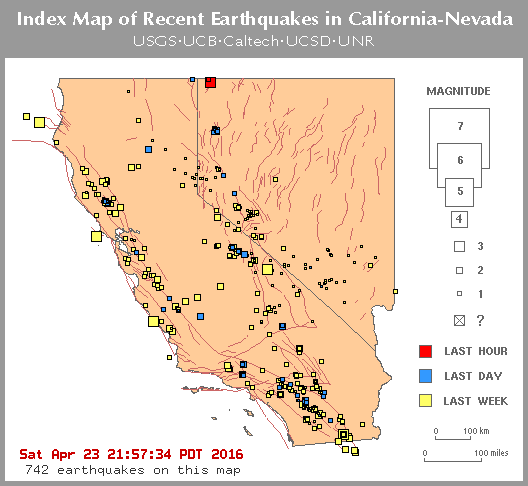
\includegraphics[width=0.5\textwidth]{recentquakes.png}
    \caption{A map showing all quakes in the week leading up to the 24th April 2016}
    \label{fig:lastweek}
\end{figure}

\begin{figure}[!h]
    \centering
    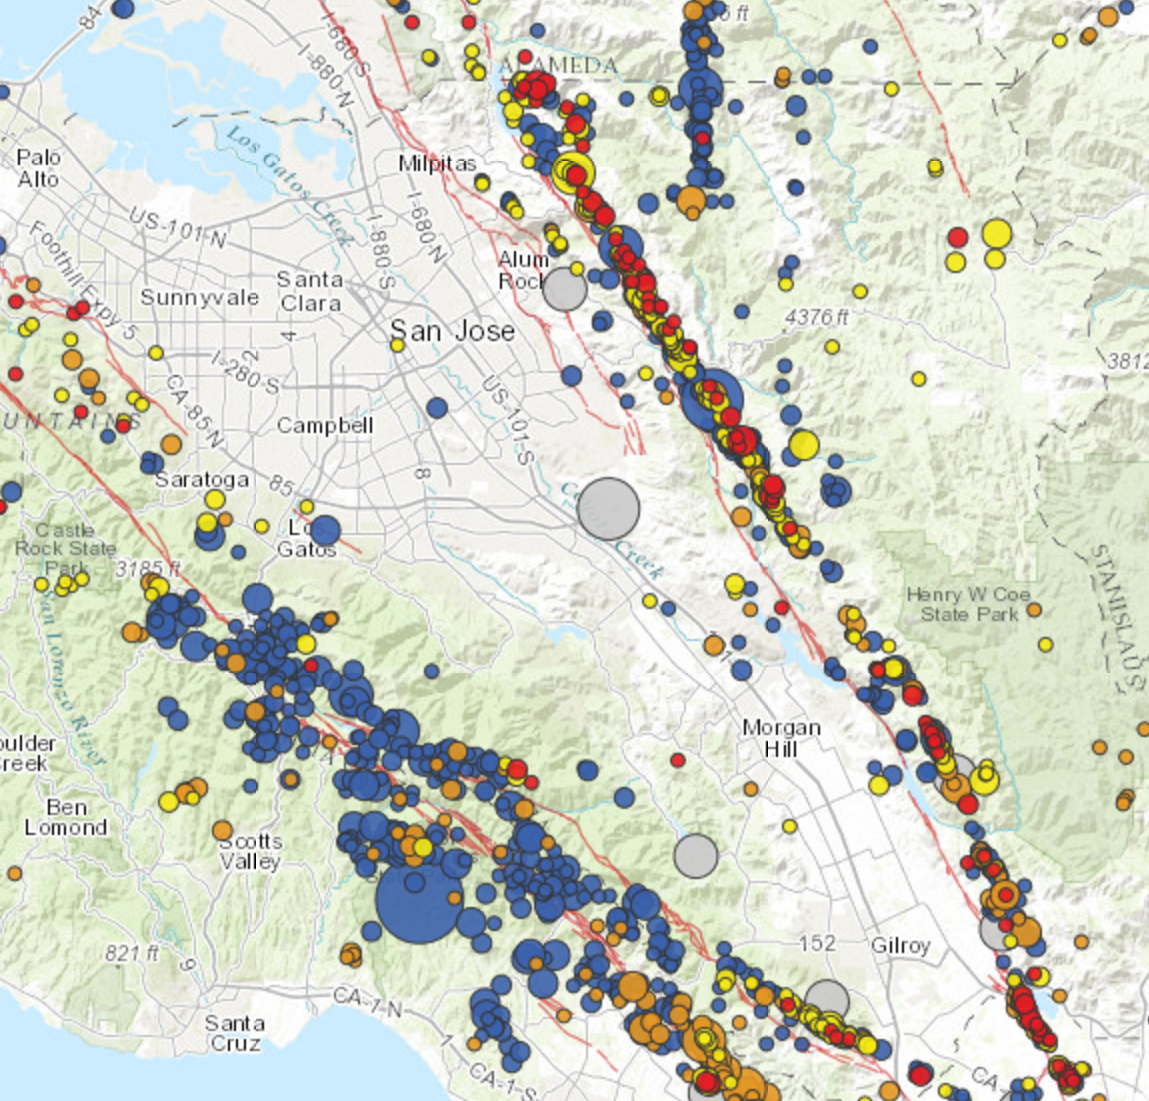
\includegraphics[width=0.5\textwidth]{bayareaquakes.PNG}
    \caption{A graphical record of all known earthquakes in much of the South Bay}
    \label{fig:baq}
\end{figure}

\section*{Works Cited}

\begin{verbatim}
Audi, T. (2016). Shaken or Stirred, This Winery Is a Big Hit With 
    Seismologists. WSJ. Retrieved 25 April 2016, from www.wsj.com/
    articles/SB125936328750267155
    
California Central Valley. (2016). AMNH. Retrieved 25 April 2016, 
    from http://www.amnh.org/explore/curriculum-collections/grace/
    grace-tracking-water-from-space/california-central-valley

Earthquakes. (2016). Earthquake.usgs.gov. Retrieved 24 April 2016, from
    http://earthquake.usgs.gov/earthquakes/map/#%7B%22feed%22%3A%227day_all%22%2C%22search%22%3Anull%2C%22listFormat%22%3A%22default%22%2C%22sort%22%3A%22newest%22%2C%22basemap%22%3A%22grayscale%22%2C%22autoUpdate%22%3Atrue%2C%22restrictListToMap%22%3Atrue%2C%22timeZone%22%3A%22utc%22%2C%22mapposition%22%3A%5B%5B31.44741029142872%2C-127.41943359375%5D%2C%5B41.86956082699455%2C-113.35693359375%5D%5D%2C%22overlays%22%3A%7B%22plates%22%3Atrue%7D%2C%22viewModes%22%3A%7B%22map%22%3Atrue%2C%22list%22%3Atrue%2C%22settings%22%3Atrue%2C%22help%22%3Afalse%7D%7D

Earthquake Facts & Earthquake Fantasy. (2016). Earthquake.usgs.gov. 
    Retrieved 25 April 2016, from http://earthquake.usgs.gov/learn/
    topics/megaqk_facts_fantasy.php
    
Gazzar, B. & Smith, K. (2016). These are California’s 5 biggest 
    vulnerabilities from a major earthquake. Sgvtribune.com. 
    Retrieved 30 April 2016, from http://www.sgvtribune.com/general
    -news/20160317/these-are-californias-5-biggest-vulnerabilities-
    from-a-major-earthquake
    
Grogan, W., & Vallerga, B. (2000). Earthquake Damage and Repair of 
    Oakland Airport Runway. J. Perform. Constr. Facil., 14(4), 
    135-140. http://dx.doi.org/10.1061/(asce)0887-3828(2000)14:4(135)

    
How Close to a Fault Do You Live?. (2016). Bayquakealliance.org. 
    Retrieved 4 April 2016, from http://bayquakealliance.org/howclose/
    
Kasarda, J. & Lindsay, G. (2011). Aerotropolis. New York: Farrar, 
    Straus and Giroux.

King, J. (2016). Loma Prieta quake left legacy of repair, renewal. 
    SFGate. Retrieved 2 May 2016, from http://www.sfgate.com/bayarea
    /article/Loma-Prieta-quake-left-legacy-of-repair-renewal-5816995.php

Krieger, L. & Gafni, M. (2016). 25 years after Loma Prieta: Bay Area 
    infrastructure is safer, but we're still on shaky ground. 
    EastBayTimes.com. Retrieved 2 May 2016, from http://www.eastbaytimes.com/
    science/ci_26710402/25-years-after-loma-prieta-bay-area-infrastructure
    
Lin II, R. (2011). Study shakes up scientists' view of San Andreas 
    earthquake risk. latimes. Retrieved 25 April 2016, from articles.
    latimes.com/2010/aug/21/local/la-me-earthquake-fault-20100821
    
Los Angeles Mayoral Seismic Safety Task Force,. (2016). Resilience 
    By Design. Los Angeles: Office of Resilience. Retrieved from
    http://www.lamayor.org/sites/g/files/wph446/f/article/files/
    Resilience%20by%20Design%20%281%29.pdf
    
Public Policy Institute of California,. (2016). California Earthquake 
    Recovery. Public Policy Institute of California. Retrieved from http://www.ppic.org/content/pubs/jtf/JTF_EarthquakeRecoveryJTF.pdf

Recent Earthquakes in California and Nevada. (2016). SCEDC.caltech.edu. 
    Retrieved 24 April 2016, from http://scedc.caltech.edu/recent/
    
Silicon Valley History. (2016). People.seas.harvard.edu. 
    Retrieved 25 April 2016, from http://people.seas.
    harvard.edu/~jones/shockley/sili_valley.html

Smith, C. (2016). What San Francisco didn't learn from the '06 quake. SFGate. 
    Retrieved 25 April 2016, from http://www.sfgate.com/homeandgarden/article/
    What-San-Francisco-didn-t-learn-from-the-06-quake-2520018.php
    
Snow, K. (2014). 25 Years After the Loma Prieta Earthquake, Are We 
    Safer?. KQED Science. Retrieved 30 April 2016, from http://ww2.
    kqed.org/science/2014/10/13/25-years-after-the-loma-prieta-
    earthquake-are-we-safer/

The Aerospace Industry in Southern California. (2016) (1st ed., pp. 10, 11). 
    Los Angeles. Retrieved from laedc.org/reports/AerospaceinSoCal_0812.pdf
\end{verbatim}

\end{document}
